\chapter{基于元学习本体增强的跨域知识表示学习模型}
跨域知识图谱的知识表示学习的关键在于如何对目标域知识图谱中的未见关系和未见实体进行嵌入。借鉴于元学习“learning to learn”的算法思想,本文通过设置多个训练任务,且在任务中模拟存在新的实体和新的关系的跨域场景。基于训练任务进行模型训练,使得模型能够学习到对未见实体和未见关系的嵌入能力。在每一个训练任务上,模型通过对关系的拓扑信息和本体信息进行学习获得对未见关系的嵌入表示,通过对未见实体邻接的关系信息聚合获得未见实体的嵌入表示。然后为了充分利用到已知关系和已知实体的特征信息,本文采用CompGCN在实例知识图谱上对所有实体和关系的初始化嵌入再进行一次更新,获得所有实体和关系最终的向量表示。最后通过多个KGE方法计算损失并进行模型优化。该模型的主要创新点如下:1)关系和实体的表示能够同时学习到事实三元组结构上的拓扑信息和本体层面上的语义信息。2)能够通过元学习的训练流程模拟出目标问题的学习任务对模型参数进行更新。3)能够同时对测试集中未见的关系和未见的实体嵌入编码。

\section{模型整体架构}
\begin{figure}[h]
  \centering
  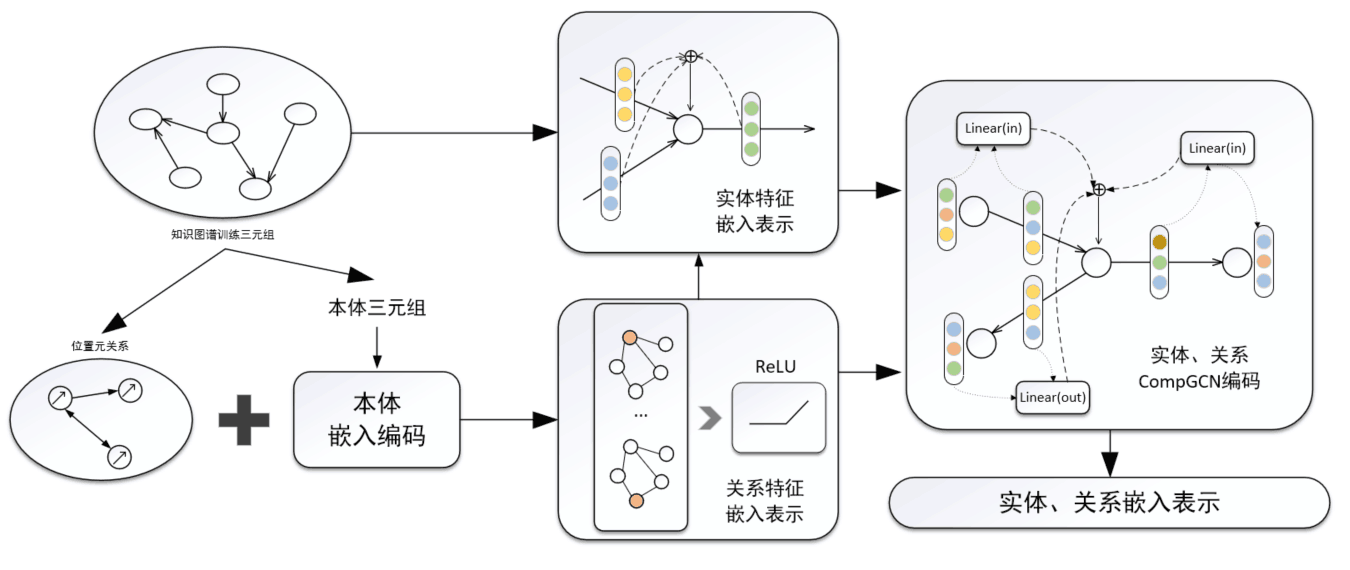
\includegraphics[width=1\textwidth]{3-1.png}
  \caption{模型架构图}
  \label{fig:3-1}
\end{figure}

本文提出的模型整体结构如图\ref{fig:3-1}所示,包含三个主要的部分:未见关系的特征嵌入、未见实体的特征嵌入以及基于元学习训练设定。为了提取关系特征,本文首先根据实例图谱中关系的相对位置结构构建了关系位置图,其中节点为实例图谱中的关系。将本体信息和关系位置图结合后,通过两层关系图卷积网络对关系的语义信息和结构信息进行更新和学习,获得关系特征的嵌入表示。为了对未见实体进行表示学习,本文对未见实体的邻接关系进行聚合,并使用关系方向特定的调整矩阵,提取所有关系的特征,以获得实体特征的初始化嵌入表示。为了利用实例图谱中的已知关系和已知实体,本文在实例图谱上采用两层复杂图卷积网络聚合所有实体和关系及其邻域特征,并对它们的嵌入表示进行更新。模型修改了复杂图卷积网络的输出层,使得关系和实体的维度不要求一致,从而可以采用多种KGE模型作为打分函数计算任务损失,来对模型进行调优。而为了能够让模型在训练过程中获得对目标域知识图谱未见实体和关系表示学习的能力,本文设置了多个训练任务对跨域场景进行模拟,在训练任务上获得最优参数,并将训练的参数用于目标域的图谱嵌入上。

对于训练集中可见的关系和实体,本文采用了传统的知识图谱表示学习的学习流程,即分别设置关系特征矩阵和实体特征矩阵,在初始化阶段对这两个矩阵按照各自目标维度随机向量初始化。在模型训练过程中通过TransE等打分函数对嵌入结果打分后进行更新,可以得到可见部分的特征嵌入。

\section{未见关系的特征嵌入}
\subsection{关系位置图构建}
为了能够与目标域知识图谱中的未见关系进行有效的特征学习,由于在源知识图谱中不存在相关的事实三元组可以提供知识,必须要从其他层面获取到对未见关系编码有效的语义信息。通过第三章,本文在本体中添加了关系的本体三元组,学习到了关系在本体层面的语义信息。同样,基于第三章的关系位置元关系的设定,可以将源域知识图谱所有的关系在关系位置图中表示,关系与关系之间通过已定义的四种关系位置元关系(tail-head,tail-tail,head-head,head-tail)进行连接。在关系位置图中,关系与关系间的位置联系可以作为关系的一种拓扑特征信息。这些结构性的信息会减少对具体实体和关系的依赖,在对关系特征进行学习的时候,通过聚合相连其他关系的信息来对关系进行特征表示,能够作用在未见的关系上。
\begin{figure}[h]
  \centering
  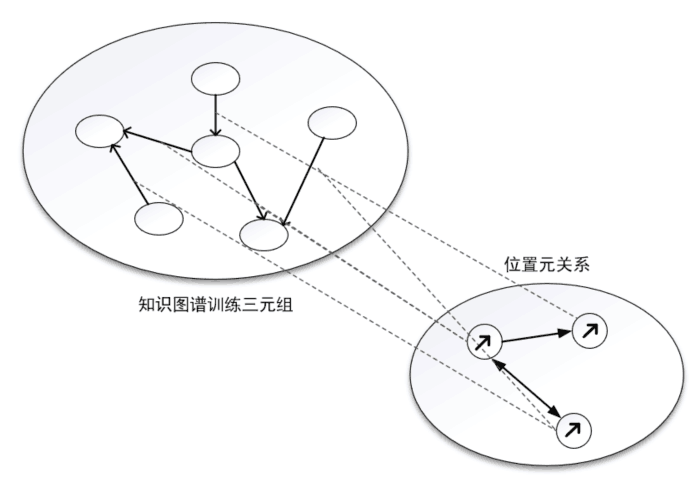
\includegraphics[width=0.5\textwidth]{3-3.png}
  \caption{从实例图构建关系图}
  \label{fig:3-3}
\end{figure}

与第三章抽取关系的位置元关系不同,在位置关系图中,本节没有对图中具有对称性的位置元关系进行筛选和去除。为了能够防止对图中对称的元关系重复的进行信息传递,在对关系节点进行特征聚合的时候,本节仅考虑每个关系节点的入向关系,以此屏蔽了位置元关系的对称性的影响。

因此根据输入的实体三元组,可以将原始的图结构转变为关系相关图,同时在构建图的过程中没有使用到任何额外的实体属性或关系属性,可以作用到任何未见或已知的关系上。在关系相关图中的节点代表关系,边表示在原始三元组任意两个关系对应的元关系。

\subsection{关系相关性系数聚合编码}
在关系位置图中,结点为原三元组中的关系,可以通过聚合关系结点的其他相邻关系结点的特征作为该关系的特征。为了能够将本体的嵌入作为对关系嵌入的语义补充,在构建好的关系位置图上,本文通过关系节点到本体概念的映射获取到各关系节点的初始化特征表示。然后通过多层图卷积网络聚合邻接节点的特征来对关系节点的特征学习,对于节点的更新公式如公式\ref{eq:4-4}所示:
\begin{equation}
  h_{v} = f\left( \sum_{(u,r) \in \mathcal{N}(v)} W h_{u}\right) \label{eq:4-4}
\end{equation}
其中\(h_{v}\)是相邻关系节点的特征。每层图卷积会有两步的操作,首先左乘归一化后的邻接矩阵对邻居节点的特征进行聚合,然后右乘一个可学习的线性转换矩阵\(W_{r}\)将输入的特征映射到目标特征空间中,最后使用一个非线性的激活函数来获取本层的特征输出。

为了在聚合关系本体信息和拓扑信息时区分不同元关系的的重要性,本文在对不同元关系连接的关系特征进行聚合时设置一个可学习的权重参数,根据任务的表现来学习不同元关系对应的重要程度,计算公式转化如公式\ref{eq:4-5}所示:
\begin{equation}
  h_{v} = f\left( \sum_{(u,r) \in \mathcal{N}(v)} W_{ dir(r) } h_{u}\right) \label{eq:4-5}
\end{equation}
其中\(W_{dir(r)}\)是两个关系节点相连的元关系类型相对应的参数,根据本文设定的四种不同的元关系,该系数由四个不同的参数控制,如公式\ref{eq:4-6}所示:
\begin{equation}
  W_{dir(r)} = \left\{ \begin{array}{rcl}
    &W_{t-h}  \mbox{,} &\quad r \in R_{tail-head} \\
    &W_{h-t}  \mbox{,} &\quad  r \in R_{head-tail} \\
    &W_{t-t}  \mbox{,} &\quad  r \in R_{tail-tail} \\
    &W_{h-h}  \mbox{,} &\quad  r \in R_{head-head} \\
    \end{array}\right\} \label{eq:4-6}
\end{equation}

\section{未见实体的特征嵌入}
\subsection{基于关系聚合的实体表示}
在仅存在源域知识图谱的一般表示学习中,知识表示学习通过对知识图谱三元组的结构信息学习,能够使得表示向量尽可能贴近事实。但在目标域知识图谱中存在未见实体的情况下,由于缺乏事实三元组的支撑,传统的KGE方法无法学习到未见实体的特征信息。

为了解决上述的问题,本文借鉴人类对未见实体的推理过程来对未见实体进行编码。如图\ref{fig:3-5}所示,传统的KGE方法能够通过对事实三元组的学习,对已知的Tom节点进行有效的学习。对于存在未见实体的目标域知识图谱,常人虽然无法获得节点X、Y、Z、A的具体内容,但是可以通过对左右两个图谱的推理可知:节点X应该是一个类似于Tom的一个学生类型的节点。因为X具有和Tom类似的邻域结构信息,如student\_of、advisor\_of及lives\_in等。这些结构性的信息可以帮助人去理解一个新的实体。同时这些实体的邻域结构信息与实体本身具体信息是无关且通用的。
\begin{figure}[h]
  \centering
  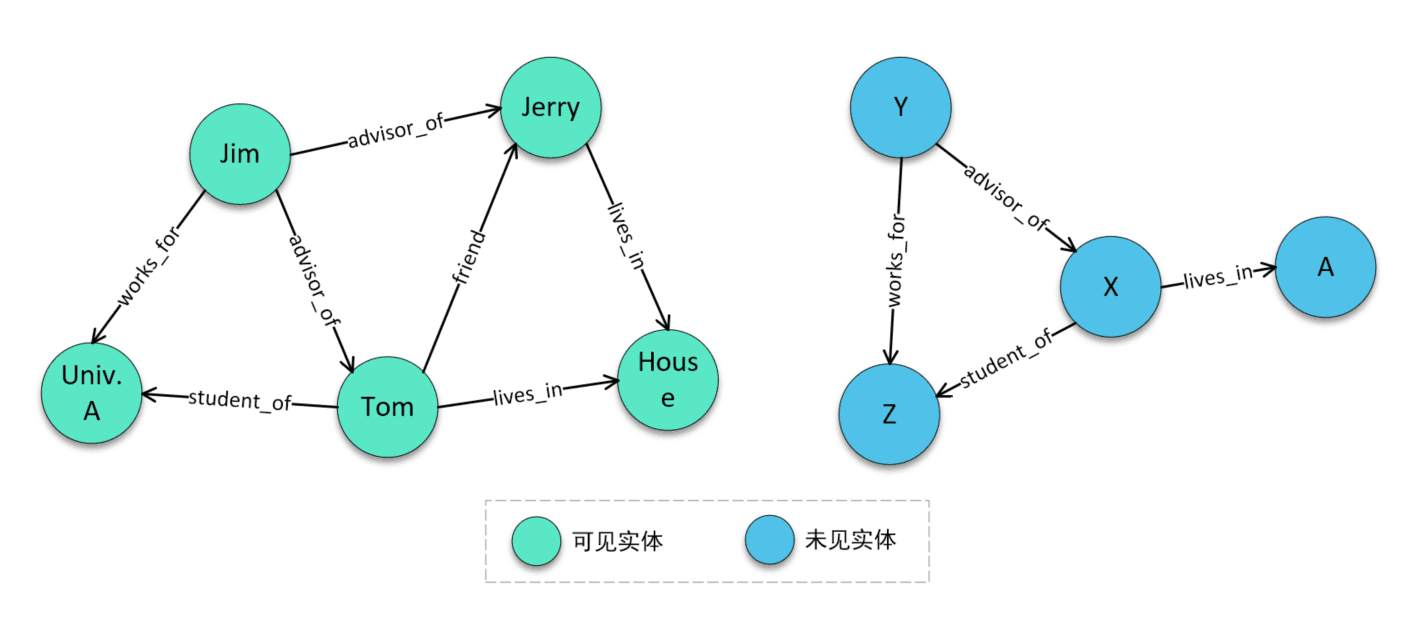
\includegraphics[width=0.8\textwidth]{3-5.png}
  \caption{未见实体的关系特征}
  \label{fig:3-5}
\end{figure}

本节通过模拟人类对于新实体的推理过程,对实体邻域的结构信息进行建模来获得实体的特征编码。实体邻域结构信息最直接的体现便是与实体直接联系的各个关系,因此本节通过使用实体相关的关系信息获得未见实体的嵌入。同时考虑到实体关系的方向性,本文通过公式\ref{eq:4-7}来进行实体关系的聚合:
\begin{equation}
  \textbf{h}_{e} = \frac{1}{|\mathcal{I}(e)| + |\mathcal{O}(e)|} \left(
    \sum_{r\in \mathcal{I}(e)}\textbf{W}_{in}^{ent} \textbf{h}_{r} +
    \sum_{r\in \mathcal{O}(e)}\textbf{W}_{out}^{ent} \textbf{h}_{r}
    \right) \label{eq:4-7}
\end{equation}
其中\(\mathcal{I}(e)\)是实体e所有连接关系中指向实体e的集合,\(\mathcal{O}(e)\)是实体e所有连接关系中由实体e出发指向其他实体的关系集合,\(\textbf{W}_{in}^{ent}\)和\(\textbf{W}_{out}^{ent}\)分别是用于在聚合实体邻接关系中入关系和出关系是对关系嵌入的权重矩阵。

然而,这种对实体通过关系聚合的方式只能对实体嵌入进行初始化表示,因为实体的邻域结构只传递类型级别的信息,而不是实例级别的信息。例如,对于节点X,我们只能推断出该节点是一个类似Tom的学生类型节点,但无法得知节点X具体是谁。为了解决这个问题,本文在下一节引入了基于GNN的实体关系联合嵌入模块,根据实体的多跳邻域结构调制每个实体和关系的初始化嵌入。

\subsection{基于GNN的实体关系联合嵌入}
在上述两个章节中,本文通过关系的本体信息和拓扑信息学习到了未见关系的初始化嵌入,通过实体的邻域结构信息的聚合学习到了未见实体的初始化嵌入。但是这些初始化的嵌入仅传递了部分的信息,如实体偏向于类型的初始化嵌入,没有充分利用到已知实体和已知关系的信息。因此,本节通过在实例知识图谱上,借鉴于CompGCN的模型结构,设计了一个能够同时对实体和关系进行邻域信息聚合的模块。该模块通过对每一个实体和关系聚合多跳邻域结构信息,能够充分利用到所有已知关系和已知实体的信息,学习到未见实体和未见关系更充分的语义表示。

该GNN网络也以CompGCN模型为基础,但是CompGCN原模型在对关系和实体进行聚合操作的时候采用了TransE、HoLE和DistMul模型的评分函数,限制了关系和实体的维度必须一致。为了能够使得该GNN网络能够输出维度不同的实体换关系的编码,本文借鉴于MaKEr\cite{chen2022meta}模型的设置,将CompGCN模型原有的实体关系聚合器修改为了一个线性转化层,可以让模型更好适应以多种传统KGE方法如RotatE来作为解码器进行下游任务,GNN层的实体嵌入更新公式如公式\ref{eq:4-8}所示:
\begin{equation}
\textbf{h}_{e}^{l+1} = f \left(
\frac{\sum_{(r,e)\in \mathcal{N}(e)}\textbf{W}_{dir(r)}^{l} [\textbf{h}_{r}^{l} ; \textbf{h}_{e}^{l}]}{|\mathcal{N}(e)|} + \textbf{W}_{self}^{l}\textbf{h}_{e}^{l}
\right) \label{eq:4-8}
\end{equation}
其中\(\mathcal{N}(e)\)是实体e的所有相连的关系集合,\(\textbf{W}_{dir(r)}^{l}\)是对集合中关系不同方向特定的权重参数,对入方向和出方向时分别记为\(\textbf{W}_{in}^{l}\)和\(\textbf{W}_{out}^{l}\),\([;]\)而指代两个向量的连接操作。\(\textbf{W}_{self}^{l}\)是针对实体e本身特征自循环更新的模型学习参数,\(f\)指代模型GNN模型的激活函数。同时,关系也在该层GCN中也进行了更新操作,如公式\ref{eq:4-9}所示:
\begin{equation}
\textbf{h}_{r}^{l+1} = \textbf{W}_{rel}^{l}\textbf{h}_{r}^{l} \label{eq:4-9}
\end{equation}

经过两层GNN网络完成了对关系嵌入和实体嵌入的更新,该模块即可输出该训练任务下所有可见的实体和关系以及未见的实体和关系的向量表示,用于本次任务的loss的计算及模型参数更新。

\section{基于元学习的训练任务设定}
为了能够对知识图谱中的未见关系和未见实体进行表示学习,借鉴于元学习“learning to learn”的思想,本文设置了训练元任务和测试元任务。训练元任务是用于训练元学习算法的任务,即在训练过程中让算法从元任务中获取经验并调整参数,以便于在测试任务中能够快速地适应。测试元任务则是在训练完成后用于测试元学习算法性能的任务。不同于元学习一般划分多个不同元任务的设定,本文采用单任务设定,即训练元任务和测试元任务均视为单一的任务。单任务设定可以使得元学习算法更加适应目标任务,并提高模型的泛化能力。同时,模型可以更加专注于学习适应固定任务的策略,还可以减少模型的计算和存储成本,并使得模型更加容易调整和解释。

本文从训练集中抽取了一系列包含未见实体和关系的训练任务来模拟跨域环境,并且在该训练环境中对模型进行训练。每个训练任务\(T^{i} = (\mathcal{E}^{i}, \mathcal{R}^{i}, \mathcal{T}^{i}_{sup},\mathcal{T}^{i}_{que})\)包含训练实体集、关系集、support训练三元组集以及query测试三元组集。为了模拟未见的组件,将部分实体和关系标记为未见,每个训练任务被重新定义为如\ref{eq:4-1}所示:
\begin{equation}
  T^{i} = (\mathcal{E}^{i} = (\hat{\mathcal{E}}^{i},\tilde{\mathcal{E}}^{i}), \mathcal{R}^{i} = (\hat{\mathcal{R}}^{i} ,\tilde{\mathcal{R}}^{i}   ), \mathcal{T}^{i}_{sup},\mathcal{T}^{i}_{que})  \label{eq:4-1}
\end{equation}
其中\(\hat{\mathcal{E}}^{i} \in \mathcal{E}^{train}\)指代实体集中的可见实体而\(\tilde{\mathcal{E}}^{i} \notin \mathcal{E}^{train}\)指代未见的实体;\(\hat{\mathcal{R}}^{i} \in \mathcal{R}^{train}\)指代关系集中的可见关系\(\tilde{\mathcal{R}}^{i} \notin \mathcal{R}^{train}\)指代未见的关系。对训练集中三元组抽取训练任务和测试任务的流程如算法\ref{alg:task}所示:
\begin{algorithm}
  \KwData{读取所有三元组,构建大图\(\mathcal{G}_{train}\)}
  \For{i < num\_subgraph}{
    选取num\_root个根节点\\
    \While{子图节点 < 50}{
      从根节点随机游走num\_step步,构建子图\(\mathcal{G}_{i}\)
    }
    从子图三元组中抽取10\%作为query三元组\\
    对query三元组中的关系和实体随机标记为未见\\
    构建support三元组中的实体和关系联系矩阵,构建关系位置图\\
    将support三元组、query三元组、关系位置图存储
  }
  \caption{任务子图构建流程}\label{alg:task}
\end{algorithm}

所有训练的总目标是基于每个任务的support集上进行对未见组件的训练使得在query集上的评估得分最高,计算函数如公式\ref{eq:4-2}所示:
\begin{equation}
  \max\limits_{ \theta } \mathbb{E} _ { T ^ { i } \sim p ( T ) } \left[ \sum\limits_{ ( h , r , t ) \in \mathcal{T} _ { \text { que } } ^ { i } } \frac { 1 } { | \mathcal{T} _ { \text { que } } ^ { i } | } \mathcal{M} ( h , r , t | \mathcal{T} _ { \text { sup } } ^ { i } ) \right] \label{eq:4-2}
\end{equation}
其中\(\mathcal{M}\)通过在support集上学习到实体和关系的嵌入表示,然后在query集上对三元组计算得分。本文采用自对抗负抽样损失函数来对计算损失更新模型,如公式\ref{eq:4-3}所示:
\begin{equation}
  \begin{aligned}
    \mathcal{L}(T^{i}) = &\frac{1}{|\mathcal{T}^{i}_{que}|} \sum\limits_{(h,r,t)\in\mathcal{T}^{i}_{que}}-log\sigma(\gamma + s(h,r,t)) \\
    &-\sum\limits_{i=1}^{n}p(h'_{i},r,t'_{i})log\sigma(-\gamma - s(h,r,t)) \label{eq:4-3}
  \end{aligned}
\end{equation}
n指代负采样的数量,\(p(h'_{i},r,t'_{i})\)指代负采样的权重系数,\(s(h,r,t)\)是用于计算嵌入向量在query三元组上的得分函数。

\section{基于链接预测任务的模型实现}
知识图谱的知识表示学习通过学习实体和关系的向量表示来捕捉隐含的语义关系和规律,跨域知识图谱的知识表示学习在传统知识表示学习的基础上,能够学习到目标域知识图谱上新的实体和关系的特征表示。为了验证知识表示学习的有效性,本文结合下游链接预测任务对提出的知识表示学习方法进行评判。

链接预测任务通常涉及知识图谱中实体对之间的关系推理。该任务基于现有事实来推断出未知的三元组,以帮助补全知识图谱中的缺失信息、推断未知实体之间的关系及预测新实体属性等。链接预测任务可分为头实体预测和尾实体预测两种类型。对于头实体预测,已知关系和一个实体,需要预测与该实体关联的另一个实体。对于尾实体预测,则是已知实体和它的某个关系,需要预测与该实体存在该关系的其他实体。为了评估模型在链接预测方面的能力,常用的指标是基于排名的,如MRR和Hits@k等。其中MRR被定义为测试数据集中每个三元组的预测排序的平均排名的倒数,而Hits@k则是指在测试数据集中每个三元组的预测概率排名中前k名的正确率,即命中率。这些指标可以帮助确定预测结果的准确性和可靠性,同时有助于对不同模型进行比较和评估。

本文在训练任务的support上学习到实体和关系的嵌入,并在query集上进行损失计算。在进行每次任务损失的过程中,通过正负样本的联合计算出损失,并以此进行梯度下降求解。负样本损失计算公式如公式\ref{eq:4-10}所示:
\begin{equation}
  \mathcal{L}_{neg} = \sum_{i = 1}^{n} \left( softmax(W[s_{tail};s_{head}])log \sigma (- [s_{tail};s_{head}]) \right) \label{eq:4-10}
\end{equation}
其中\(s_{tail}\)和\(s_{head}\)是对一个测试三元组对应的尾结点负采样得分和头结点负采样得分,n代表负采样的数量,\([;]\)操作将正负样本的得分矩阵进行简单的连接操作,\(W\)是对得分进行微调的权重参数,本文默认设置为1。之后和正样本的得分求得算术平均即为该测试三元组的单个损失。

对于模型的训练流程,本文按照元学习单任务训练方法进行,每个任务的目标都是使该任务下的连接预测效果最优,单个任务的训练流程包含有5步::

\begin{enumerate}[label=\arabic*)]
  \item 初始化模型参数,主要包含了训练数据集中可见实体和关系的嵌入初始化、元关系的权重参数以及两个不同阶段的GCN层和CompGCN层的传递参数。
  \item 获得任务的支持集和查询集,主要从原训练集中抽取单个任务的子图,并划分为支持集和查询集,同时对关系和节点的标签进行设置以模拟出未见组件。
  \item 单次任务训练获得实体关系的嵌入,通过KGE模型计算查询集损失,通过损失函数进行梯度下降求解。
  \item 更新模型参数,重复下一个任务的训练直至效果不再更优。
  \item 对测试集进行模型测试,输出任务得分。
\end{enumerate}

\section{本章小结}
本章从本文模型的总体架构开始,详细介绍了模型的各个组成部分,包括主要的未见关系嵌入、未见实体嵌入以及基于元学习的训练任务设定和基于链接预测任务的模型实现的说明。对未见关系嵌入,说明了本文模型如何对关系的拓扑结构进行提取以及如何通过图卷积层对关系的本体信息和拓扑信息进行联合学习,从而获得未见关系的有效表示;对未见实体嵌入,通过未见实体的邻接关系的特征聚合,并且在实例知识图谱上通过GNN来聚合其他关系和实体信息,完成最后的实体和关系的特征更新。之后的章节中将对本文模型在测试数据集上进行充分的实验,检验本文模型的有效性。